Several iterations were required to get proper adjustments to the LSTM model for candlestick data and KNN for the NLP processing. The iterations involved observing the loss function through the deep learning model using TensorBoard and analyzing its precision, overfitting and underfitting on both models.

\subsection{Cryptocurrency data set training and tuning }

The final adjustments for the training of the neural network can be seen in [12]. The neural network implementation, training and performance for every cryptocurrency trained on the spark environment can be visualized as well in the provided citation. Each candlestick data set is processed in a pandas DataFrame. The loss function and window offset (period in which the neural network predicts the values based on past data) were carefully chosen to approximate the prediction as much as possible for all the sets. Primarily, it was observed that on average most of the models adapt properly at 300 epochs\footnote{The number of epochs is a hyperparameter that defines the number times that the learning algorithm will work through the entire training data set\cite{brownlee_when_2018}}  with “Mean Square Error” as loss function and 256 neurons on 3 layers (one hidden). The model can mutate, and it is let to the reader to try to find a better tuning mechanism. It is important to highlight that for the given model the data set was aggregated to present hourly data instead of minute. The reason for this was for the expensive of the process and the amount of resources a training model takes for a single currency. In more powerful environments the model can mutate to observe minute predictions.

\begin{figure}[H]
   \centering
   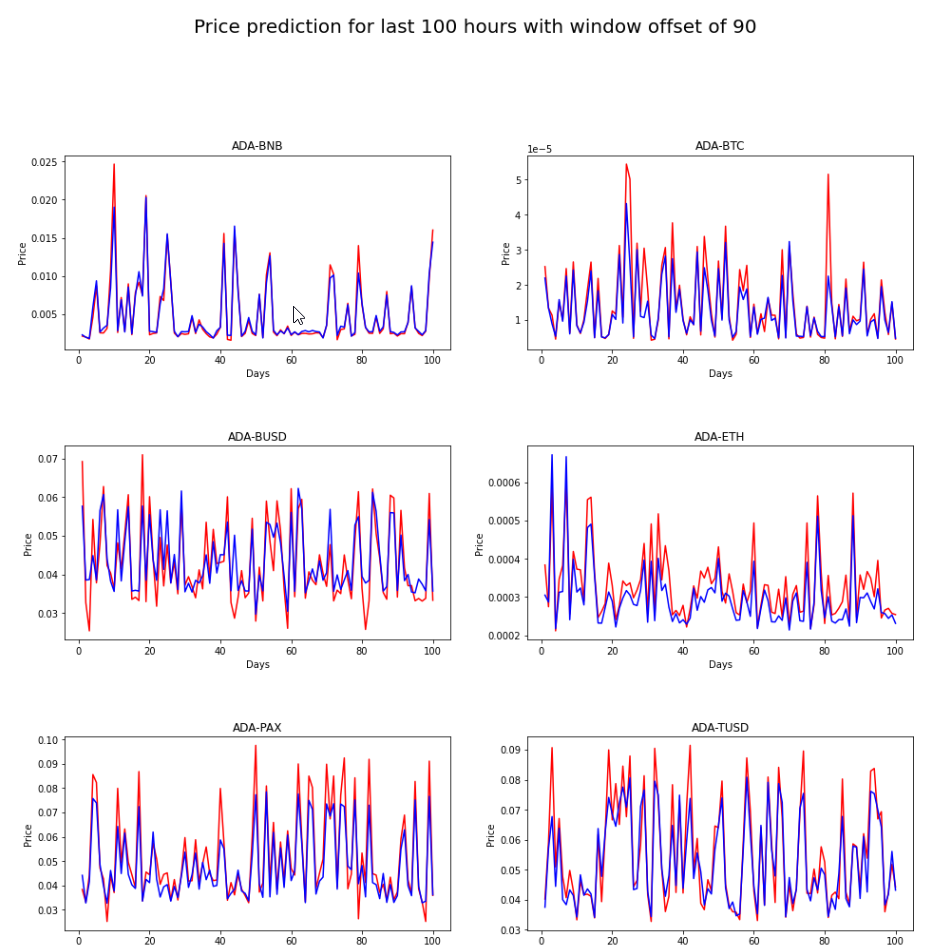
\includegraphics[width=\linewidth]{fig/MLCryptoChart.png}
    \caption{Different predictions after the model has been trained}
    \label{fig:MLCryptoChart}
\end{figure}

\subsection{Newsfeed data set training and tuning}

Trying to tune and adjust the newsfeed data set was even more complicated. The KNN algorithm was used under the premise that as the number of clusters grow for the model to be trained, more differences can be spotted after text processing. The distances between the clusters should increase and get to a state enough to assert and properly distinguish the topics for the articles. On the other hand, a normal sentiment analysis from previously trained models were made just to visualize how much the algorithms could predict the positive or negative impact on specific articles. It was however not possible to segregate the clusters to a distance considerable enough to define topics on the news. This is a limitation addressed in the next section.

\begin{figure}[H]
   \centering
   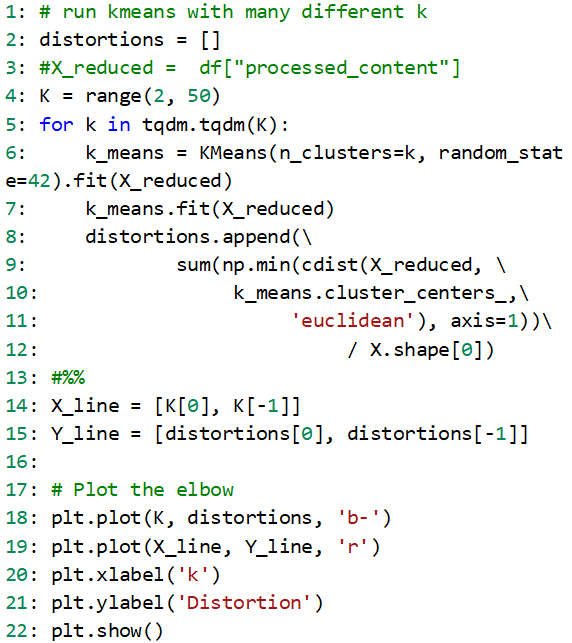
\includegraphics[width=\linewidth]{fig/TextAnalysisDistorions.png}
    \caption{Code snippet to determine the best number of clusters}
    \label{fig:TextAnalysisDistorions}
\end{figure}

\begin{figure}[H]
   \centering
   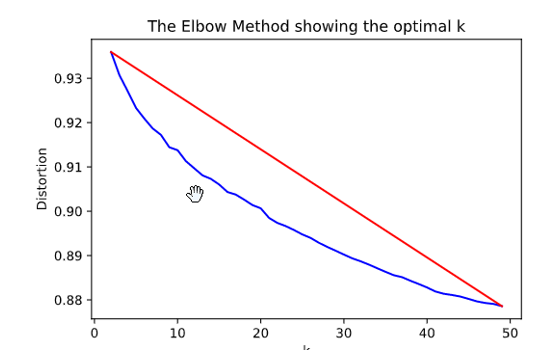
\includegraphics[width=\linewidth]{fig/DistorionChart.png}
    \caption{Results plot to determine proper number of clusters}
    \label{fig:DistorionChart}
\end{figure}


After executing the code from \ref{fig:DistorionChart}, the results to determine a suitable distance between clusters was performed. It was not possible to find a proper distinction between the news, the best fit for KNN cluster classification was 2, which is not suitable for the problem to solve. As the number of clusters increase, it is evident the classification algorithm is not able to distribute properly information among different groups, and therefore different approaches must be performed.

